\documentclass[11pt,a4paper]{article}

\usepackage[utf8]{inputenc}
\usepackage[english]{babel}
\usepackage[T1]{fontenc}
\usepackage{amsmath, amssymb}
\usepackage{graphicx}
\usepackage{booktabs} 
\usepackage{xcolor}
\usepackage{hyperref}
\usepackage{listings}
\usepackage{parskip} 
\usepackage{setspace}
\usepackage{svg}
\setstretch{1.15}  
\usepackage[a4paper,top=2cm,bottom=2cm,left=3cm,right=3cm]{geometry}

\hypersetup{colorlinks=true,linkcolor=blue,filecolor=magenta,urlcolor=cyan}

\definecolor{githubcolor}{RGB}{0, 131, 209}

\lstset{basicstyle=\ttfamily\small,breaklines=true,frame=single,backgroundcolor=\color{gray!10}}


\title{
    \vspace{-2cm}
    \vspace{0.5cm}
    \Huge Solving the Traveling Salesperson Problem (TSP) using Evolutionary Computation \\
    \vspace{1cm}
    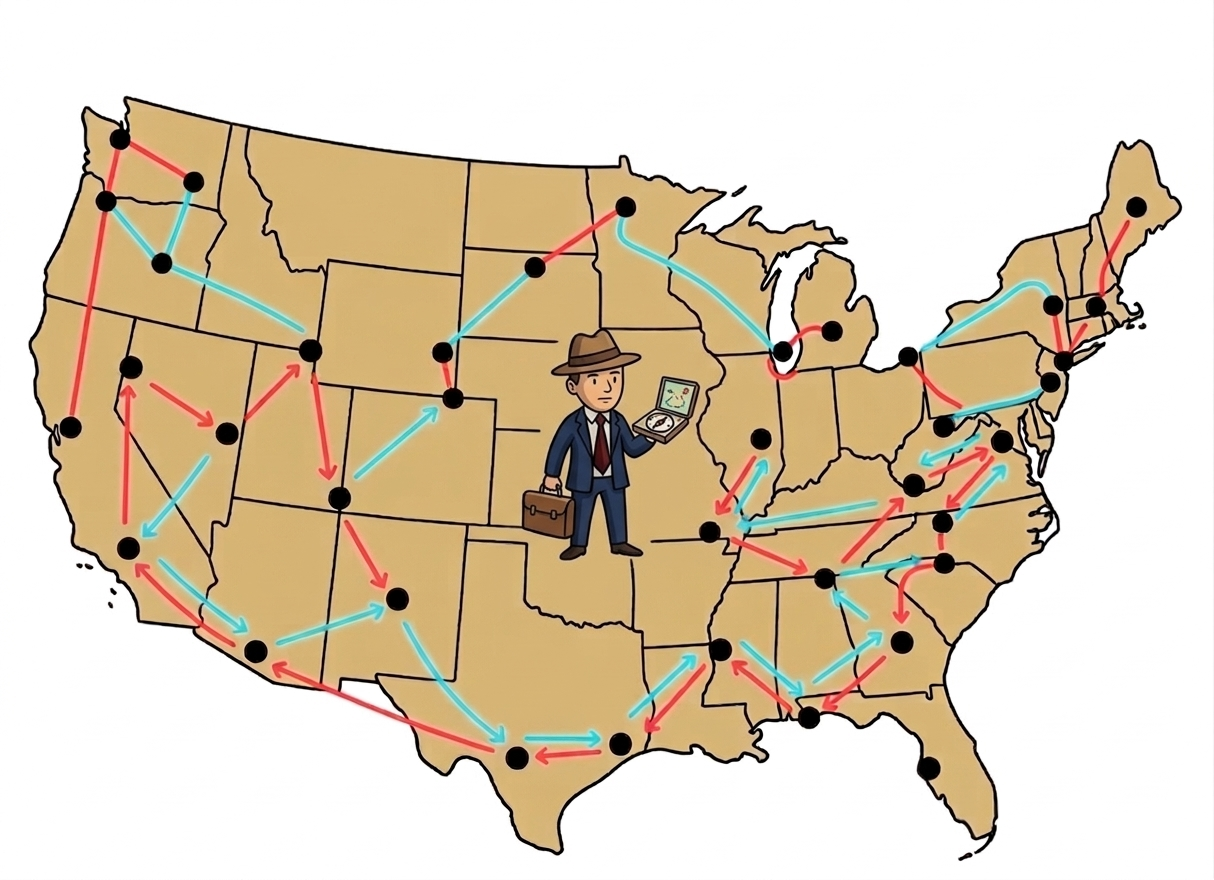
\includegraphics[width=1.0\textwidth, height=15cm, keepaspectratio]{assets/TSP_report_cover_image.png} \\
    \vspace{0.5cm}
}

\author{\href{https://github.com/javierruanohdez}{\textbf{\color{githubcolor}Javier Ruano Hernández}}}

\date{\today}

\begin{document}
\frenchspacing

\maketitle

\begin{abstract}
\noindent
This study addresses the Traveling Salesperson Problem (TSP) using Genetic Algorithm (GA) techniques. A comparative analysis is conducted between a baseline approach (OX1 Crossover and Swap Mutation) and an improvement proposal oriented toward adjacency preservation (Edge Recombination Crossover and Inversion). The results demonstrate that transitioning from an order-based logic to an edge-based logic improves convergence efficiency by up to 1000\% on the 48-city dataset.
\end{abstract}

\newpage

\section{Introduction}
The Traveling Salesperson Problem (TSP) is a classic combinatorial optimization challenge classified as NP-hard. This project implements an Evolutionary Computation environment in Python to minimize the traveled distance in a 48-city route, simulating natural selection processes: crossover, mutation, and survival of the fittest.

\subsection{Study Objective}
The main objective is to reach an optimal solution defined by a total distance traveled $D \le 35,000.00$ units, analyzing the algorithm's sensitivity to variations in population critical mass and mutation rate.

\section{Experimental Setup}
The experiment was developed in a \textit{Jupyter Notebook} environment using standard \texttt{Python} libraries (\texttt{NumPy}, \texttt{Random}, \texttt{Matplotlib}). The fundamental hyperparameters are detailed in Table \ref{tab:hiperparametros}.

\begin{table}[h!]
\centering
\caption{Experimental Setup Parameters}
\label{tab:hiperparametros}
\begin{tabular}{@{}ll@{}}
\toprule
\textbf{Parameter} & \textbf{Description} \\ \midrule
\texttt{population\_size} & Number of individuals (routes) in each generation. \\
\texttt{num\_generations} & Maximum iteration limit (set to 2000). \\
\texttt{mutation\_rate} & Probability of genetic alteration for diversity. \\
\textbf{Stopping Criterion} & Distance $\le 35,000.00$ or iteration exhaustion. \\ \bottomrule
\end{tabular}
\end{table}

\section{Parametric Study: Original Algorithm}
Convergence was analyzed by varying the population in the $[100, 1000]$ range and mutation in $[0.2, 0.4, 0.6]$. The baseline model uses:
\begin{itemize}
    \item \textbf{Order 1 Crossover (OX1):} Preservation of relative order via toroidal logic.
    \item \textbf{Swap Mutation:} Random swapping of two alleles (cities).
\end{itemize}

\subsection{Convergence Observations}
Statistical analysis reveals a highly stochastic nature. Low mutation rates ($0.2$) were identified as prone to getting trapped in local optima due to an excessively conservative character. Curiously, the $0.6$ rate showed greater success by introducing the necessary chaos to explore new regions of the search space, compensating for the inefficiency of the \textit{Swap} operator in long routes.

\includesvg[width=1.0\textwidth]{results/original_algorithm_tsp_convergence.svg} \\

\section{Improvement Proposal: Adjacency Approach}
Upon detecting the instability of the OX1 model, a paradigm shift toward edge preservation is proposed.

\subsection{Edge Recombination Crossover (ERX)}
The ERX operator constructs an \textit{Edge Table} to prioritize inheriting direct connections. The smart selection of the next node is based on the principle of the fewest remaining edges, ensuring that the offspring inherits between 95\% and 99\% of the parental edges.

\subsection{Inversion Mutation}
Unlike \textit{Swap}, which breaks up to 4 connections, inversion only alters 2, acting as a local search optimizer that untangles route segments without destroying the global structure.

\section{Results and Conclusions}
The comparison between the baseline model and the proposed one (\textit{ERX + Inversion}) yields the following technical conclusions:

\begin{enumerate}
    \item \textbf{Convergence Efficiency:} The proposed model reaches the target fitness between generations 125 and 330, compared to the 2000 required by the baseline model.
    \item \textbf{Robustness:} The proposal demonstrates independence from critical mass; even with a population of 100 individuals, the algorithm is capable of converging, representing a 90\% computational saving.
    \item \textbf{Stability:} The convergence curves of the proposed model are predictable, indicating minimal reliance on chance once a high-quality adjacency inheritance is established.
\end{enumerate}

\includesvg[width=1.0\textwidth]{results/proposed_vs_original_algorithm_tsp_convergence.svg} \\

\begin{thebibliography}{9}
\bibitem{erx_web} 
\textit{Edge Recombination Crossover (ERX)}. Resource used for the pseudocode approach and adjacency logic of the proposed improvement algorithm. Available at:\\ \url{https://k78ma.github.io/quartz/4B/ECE-457A/Edge-Recombination-Crossover}
\end{thebibliography}

\end{document}